\documentclass[11pt, a4paper, twoside, openright]{book}
\usepackage{subfiles}

% Babel
\usepackage[english]{babel}

% Font
\usepackage[utf8]{inputenc}
\usepackage[T1]{fontenc}
\usepackage{amssymb,amsmath,amsthm,amsfonts}
\usepackage{eucal}
\usepackage{textcomp}

% Footnote


% Hyperref
\usepackage[hyphens]{url}
\usepackage{cite}
\usepackage{hyperref}
\usepackage{nameref}
\usepackage{url}
% Images
\usepackage[pdftex]{graphicx}
	%\usepackage{subfigure}
\usepackage{subfig}
\usepackage{eso-pic}
\usepackage{caption}
\usepackage{wrapfig}

% List
\usepackage{enumerate}

% SI units
\usepackage{siunitx}

% Standalone
\usepackage[subpreambles=true]{standalone}
\usepackage{import}

% Tables
\usepackage{tabularx}
\usepackage{booktabs}
\usepackage{multirow}


% Typeset
%\usepackage[top=2cm,bottom=2cm,left=2cm,right=2cm]{geometry}
\usepackage[top=2cm,bottom=2cm,left=2cm,right=2cm]{geometry}
\usepackage{fancyhdr}
\usepackage{indentfirst}
\usepackage{titlesec}
\usepackage{setspace}
\usepackage{xspace}
% \usepackage{parskip}  % Elimina il separatore a inizio paragrafo
\usepackage{afterpage}
\usepackage{comment}



%Per scrivere matrice identità
\usepackage{bbold}
%Per semplificazione formule
\usepackage{cancel}

%Evidenziare formule
\usepackage{empheq}
	%oppure
	%\usepackage{xcolor}
\usepackage{soul}

%Display data
\usepackage{datetime}

%Physics
\usepackage{physics}

%%
\captionsetup[table]{font=small,labelfont={bf},skip=10pt}
\captionsetup[figure]{font=small,labelfont={bf},skip=10pt}

%intestazione pagina
%\pagestyle{fancy}
%\fancyhf{}
%\fancyhead[RE]{\ifnum\value{chapter}>0\nouppercase{\leftmark}\fi}
%\fancyhead[LE]{\small\textbf{\thepage}}
%\fancyhead[LO]{\nouppercase{\rightmark}}
%\fancyhead[RO]{\small\textbf{\thepage}}
%\renewcommand{\headrulewidth}{0.0pt}
%\renewcommand{\footrulewidth}{0.0pt}



%link ipertestuale per indice
\hypersetup{
	colorlinks=false,
	linkcolor=black,
	filecolor=blue,
	citecolor = blue,
	urlcolor=blue,
	}

%%%%%indent%%%
\setlength{\parindent}{0pt}
\setlength{\parskip}{0pt}

%boh
%\renewcommand{\chaptermark}[1]{%
% \markboth{\MakeUppercase{%
% \chaptername}\ \thechapter.%
% \ #1}{}}

% Derivatives
\renewcommand{\d}[0]{\mathrm{d}}
\newcommand{\dev}[2]{\displaystyle \frac{\d #1}{\d #2}}
\newcommand{\pdev}[2]{\displaystyle \frac{\partial #1}{\partial #2}}
\newcommand{\ndev}[3]{\displaystyle \frac{\d^{#3} #1}{\d #2^{#3} } }
\newcommand{\npdev}[3]{\displaystyle \frac{\partial^{#3} #1}{\partial #2^{#3} } }


%% Norms
\newcommand{\absvec}[1]{| \vec{#1} |}
\newcommand{\normvec}[1]{|\!| \vec{#1} |\!|}

\newcommand{\vmed}[1]{\left \langle #1 \right \rangle}
\newcommand{\vmedvec}[1]{\langle #1 \rangle}
\newcommand{\R}[0]{\mathbb{R}}
\renewcommand{\H}[0]{\operatorname{H}}

%Evidenziare formule
\newcommand{\mathcolorbox}[2]{\colorbox{#1}{$\displaystyle #2$}}
\newcommand{\hlfancy}[2]{\sethlcolor{#1}\hl{#2}}


%%%%%%%%%%%%%%%%%%%%Theorem, Corollary, Lemma, Proposition%%%%%%%%%%%%%%%%%
\usepackage[many,most,theorems]{tcolorbox}

\newtcbtheorem{theorem}{Theorem}{ % frame stuff
    boxrule = 1pt,
    breakable,
    enhanced,
    frame empty,
    interior style= {orange!20},
    %interior empty,
    colframe=black,
    borderline ={1pt}{0pt}{black},
    left=0.2cm,
    % title stuff
    attach boxed title to top left={yshift=-2mm,xshift=0mm},
    coltitle=black,
    fonttitle=\bfseries,
    colbacktitle=white,
    fontupper=\slshape,
    boxed title style={boxrule=1pt,sharp corners}}{theorem} 

\newtcbtheorem{corollary}{Corollary}{ % frame stuff
    boxrule = 1pt,
    breakable,
    enhanced,
    frame empty,
    interior style= {orange!20},
    %interior empty,
    colframe=black,
    borderline ={1pt}{0pt}{black},
    left=0.2cm,
    % title stuff
    attach boxed title to top left={yshift=-2mm,xshift=0mm},
    coltitle=black,
    fonttitle=\bfseries,
    colbacktitle=white,
    fontupper=\slshape,
    boxed title style={boxrule=1pt,sharp corners}}{corollary} 
    
\newtcbtheorem{lemma}{Lemma}{ % frame stuff
    boxrule = 1pt,
    breakable,
    enhanced,
    frame empty,
    interior style= {orange!20},
    %interior empty,
    colframe=black,
    borderline ={1pt}{0pt}{black},
    left=0.2cm,
    % title stuff
    attach boxed title to top left={yshift=-2mm,xshift=0mm},
    coltitle=black,
    fonttitle=\bfseries,
    colbacktitle=white,
    fontupper=\slshape,
    boxed title style={boxrule=1pt,sharp corners}}{lemma} 


%%%%%%%%%%%%%%%%%%%%Definition%%%%%%%%%%%%%%%%%


\newtcbtheorem{definition}{Definition}{ % frame stuff
    boxrule = 1pt,
    breakable,
    enhanced,
    frame empty,
    interior style= {blue!10},
    %interior empty,
    colframe=black,
    borderline ={1pt}{0pt}{black},
    left=0.2cm,
    % title stuff
    attach boxed title to top left={yshift=-2mm,xshift=0mm},
    coltitle=black,
    fonttitle=\bfseries,
    colbacktitle=white,
    boxed title style={boxrule=1pt,sharp corners}}{definition} 


%\theoremstyle{definition}
%\newtheorem{definition}{Definition}%[section]



%%%%%%%%%%%%%%%%%%%%Exercise and example%%%%%%%%%%%%%%%%%

\newtcbtheorem{exercise}{Exercise}{ % frame stuff
    boxrule = 1pt,
    breakable,
    enhanced,
    frame empty,
    interior style= {blue!6},
    %interior empty,
    colframe=black,
    borderline ={1pt}{0pt}{black},
    left=0.2cm,
    % title stuff
    attach boxed title to top left={yshift=-2mm,xshift=0mm},
    coltitle=black,
    fonttitle=\bfseries,
    colbacktitle=white,
    boxed title style={boxrule=1pt,sharp corners}}{exercise} 

\newtcbtheorem{example}{Example}{ % frame stuff
    boxrule = 1pt,
    enhanced,
    frame empty,
    interior style= {green!6},%{left color=yellow!70,right color=green!70},
    %interior empty,
    colframe=black,
    borderline ={1pt}{0pt}{black},
    breakable,
    left=0.2cm,
    % title stuff
    attach boxed title to top left={yshift=-2mm,xshift=0mm},
    coltitle=black,
    fonttitle=\bfseries,
    colbacktitle=white,
    boxed title style={boxrule=1pt,sharp corners}}{example}
  
%\newtheorem{exercise}{Exercise}
%\newtheorem{example}{Example}

%%%%%%%%%%%%%%%%%%%%%%%%%%%%%%%%%%%

\theoremstyle{remark}
\newtheorem*{remark}{Remark}
\newtheorem{observation}{Observation}
%Evidenziare testo
\newtheorem*{solution}{Solution}

\newcommand\mybox[1]{%
  \fbox{\begin{minipage}{0.9\textwidth}#1\end{minipage}}}

  %Spiegazioni/verifiche
\newenvironment{greenbox}{\begin{mdframed}[hidealllines=true,backgroundcolor=green!20,innerleftmargin=3pt,innerrightmargin=3pt,innertopmargin=3pt,innerbottommargin=3pt]}{\end{mdframed}}

\newenvironment{bluebox}{\begin{mdframed}[hidealllines=true,backgroundcolor=blue!10,innerleftmargin=3pt,innerrightmargin=3pt,innertopmargin=3pt,innerbottommargin=3pt]}{\end{mdframed}}

\newenvironment{yellowbox}{\begin{mdframed}[hidealllines=true,backgroundcolor=yellow!20,innerleftmargin=3pt,innerrightmargin=3pt,innertopmargin=3pt,innerbottommargin=3pt]}{\end{mdframed}}

\newenvironment{redbox}{\begin{mdframed}[hidealllines=true,backgroundcolor=red!20,innerleftmargin=3pt,innerrightmargin=3pt,innertopmargin=3pt,innerbottommargin=3pt]}{\end{mdframed}}

\newenvironment{orangebox}{\begin{mdframed}[hidealllines=true,backgroundcolor=orange!20,innerleftmargin=3pt,innerrightmargin=3pt,innertopmargin=3pt,innerbottommargin=3pt]}{\end{mdframed}}

%emph equation
\newcommand*\myyellowbox[1]{%
  \colorbox{yellow!40}{\hspace{1em}#1\hspace{1em}}}

\newcommand*\mygreenbox[1]{%
  \colorbox{green!20}{\hspace{1em}#1\hspace{1em}}}
  

%%%%%%%%%%PROOF%%%%%%%%%%%%%%%%%%%%%%%%%%%%%
\usepackage{xpatch}
\xpatchcmd{\proof}{\itshape}{\normalfont\proofnamefont}{}{}
\newcommand{\proofnamefont}{\bfseries}
\renewcommand\qedsymbol{$\blacksquare$}  
  







%\usepackage{eso-pic}
%
%\newcommand\BackgroundPic{%
%\put(0,0){%
%\parbox[b][\paperheight]{\paperwidth}{%
%\vfill
%\centering
%\includegraphics[scale=1.5]{../frontespizio/back.jpg}%
%\vfill
%}}}

%\includegraphics[width=1.4\paperwidth,height=\paperheight,%
%keepaspectratio]{../frontespizio/back.jpg}%


\begin{document}

%%%%%%FRONTESPIZIO%%%%%%
%Reset the geometry of frontespizio
\newgeometry{inner=20mm,
            outer=20mm,% = marginparsep + marginparwidth
                       %   + 5mm (between marginpar and page border)
            top=20mm,
            bottom=20mm,
            marginparsep=6mm,
            marginparwidth=30mm}
\makeatletter
\renewcommand{\@marginparreset}{%
  \reset@font\small
  \raggedright
  \slshape
  \@setminipage
}
\makeatother


\frontmatter

\pagecolor{blue} %Page color blue!70
%%%%%%FRONTESPIZIO%%%%%%


%%%%%%FRONTESPIZIO%%%%%%


\begin{titlepage} % Suppresses headers and footers on the title page
	
	%Wallpaper
	%\AddToShipoutPicture*{\BackgroundPic}
	%%%\AddToShipoutPicture*{\put(-8,0){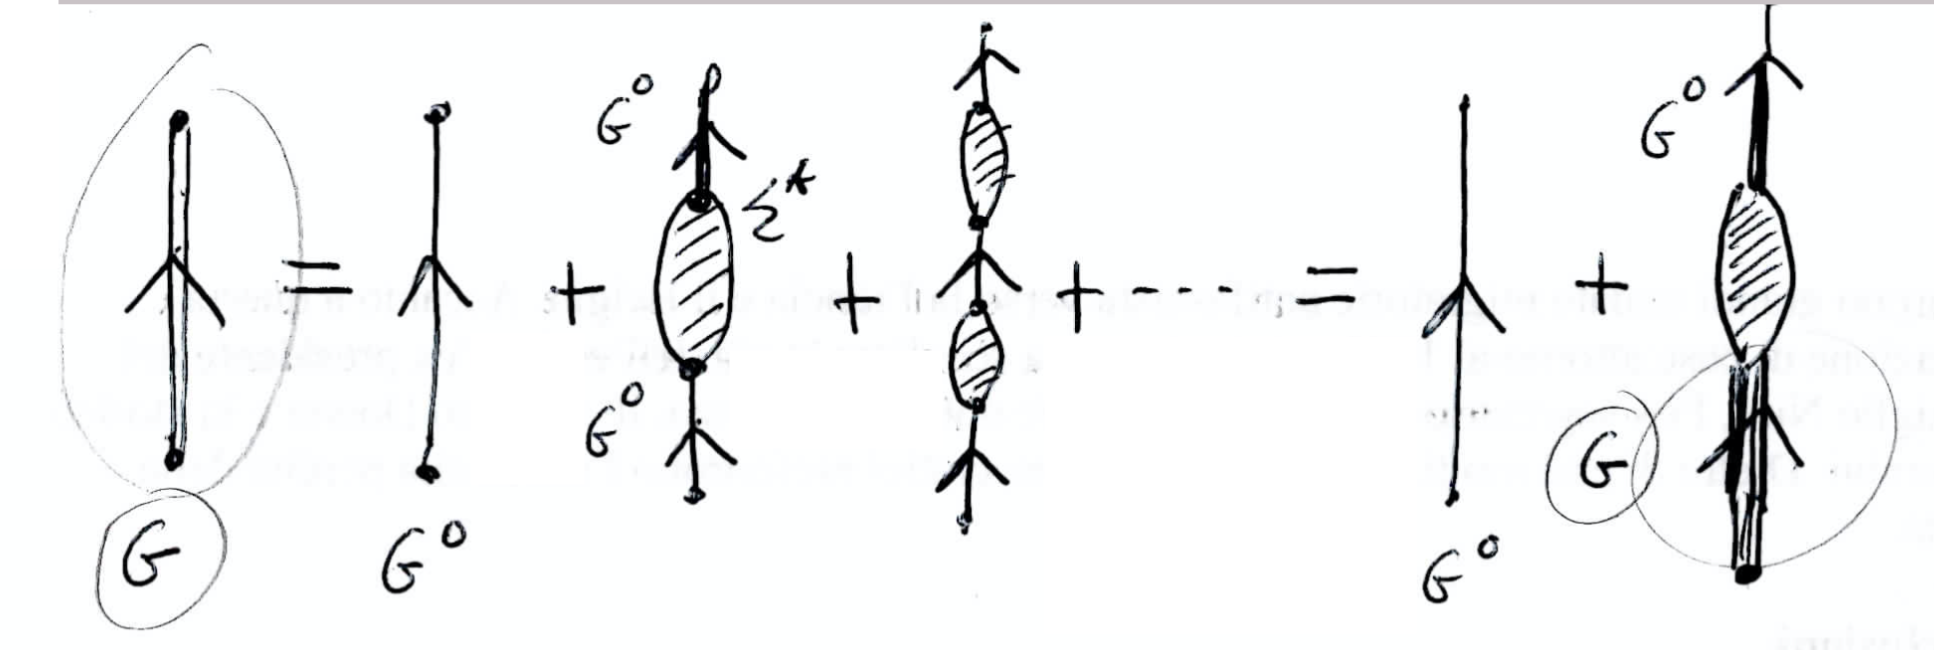
\includegraphics[scale=0.4]{../frontespizio/4.jpeg}}} % Image background
	
	\centering % Centre everything on the title page
	
	\scshape % Use small caps for all text on the title page
	
	\vspace*{\baselineskip} % White space at the top of the page
	
	%------------------------------------------------
	%	Title
	%------------------------------------------------
	
	\rule{\textwidth}{1.6pt}\vspace*{-\baselineskip}\vspace*{2pt} % Thick horizontal rule
	\rule{\textwidth}{0.4pt} % Thin horizontal rule
	
	\vspace{0.75\baselineskip} % Whitespace above the title
	
	\textcolor{black}{\large LECTURE NOTES\\ OF\\ \LARGE \textbf{INTRODUCTION TO NANOPHYSICS}\\} % Title
	
	\vspace{0.75\baselineskip} % Whitespace below the title
	
	\rule{\textwidth}{0.4pt}\vspace*{-\baselineskip}\vspace{3.2pt} % Thin horizontal rule
	\rule{\textwidth}{1.6pt} % Thick horizontal rule
	
	\vspace{2\baselineskip} % Whitespace after the title block
	
	%------------------------------------------------
	%	Subtitle
	%------------------------------------------------
	
	\textcolor{black}{Collection of the lectures notes of professor Giovanni Mattei.} % Subtitle or further description
	
	\vspace*{3\baselineskip} % Whitespace under the subtitle
	
	%------------------------------------------------
	%	Editor(s)
	%------------------------------------------------
	
	\textcolor{black}{Edited By}
	
	\vspace{0.5\baselineskip} % Whitespace before the editors
	
	\textcolor{black}{\scshape\Large Alice Pagano, Martina Russo, Rachele Favaretto, Alessandra Sabatti \\} % Editor list
	
	\vspace{0.5\baselineskip} % Whitespace below the editor list
	
	\textcolor{black}{\textit{The University of Padua } }% Editor affiliation
	
	\vspace{0.5\baselineskip}
	
	\textcolor{black}{\small Academic year 2019-2020}
	
	\vspace{1cm}
	
	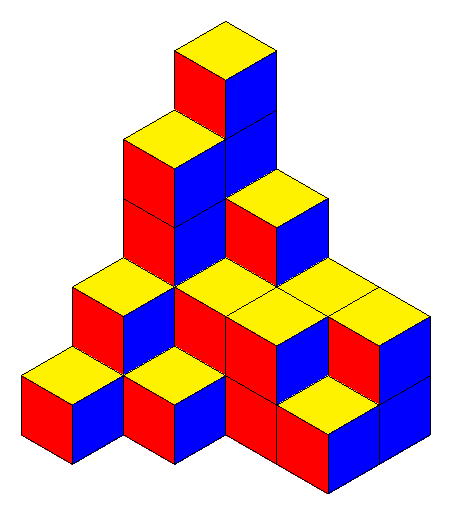
\includegraphics[width=10cm]{../frontespizio/3.pdf}
	
	\vspace{1cm}
	
	\textcolor{black}{Source available: \url{https://github.com/AlicePagano/}
	\vspace{1cm}}
	
	\textcolor{black}{\footnotesize Compiled: \today} % Editor affiliation
	

\end{titlepage}

\clearpage{\pagestyle{empty}\cleardoublepage}













\pagecolor{white}

%%%ABSTRACT%%%%%%%%%

\chapter*{\centering {\normalsize Abstract}}
\noindent In this document I have tried to reorder the notes of the “Introduction to Many-Body Theory” course held by Professor Pier Luigi Silvestrelli at the Department
of Physics of the University of Padua during the second semester of the 2019-20 academic year of the master's degree.
%The notes are \textbf{fully} integrated with the material provided by the professor in the Moodle platform. 
%In addition, I will integrate them, as best as possible, with the books recommended by the professor.
There may be formatting errors, wrong marks, missing exponents etc. If you find errors, let me know (alice.pagano@studenti.unipd.it) and I will correct them, so that this document can be a good study support.

\vspace{1cm}
\noindent Padova, \today  \hspace{6cm} Alice Pagano

\tableofcontents


\pagestyle{plain}



\newgeometry{inner=20mm,
            outer=49mm,% = marginparsep + marginparwidth
                       %   + 5mm (between marginpar and page border)
            top=20mm,
            bottom=25mm,
            marginparsep=6mm,
            marginparwidth=30mm}
\makeatletter
\renewcommand{\@marginparreset}{%
  \reset@font\small
  \raggedright
  \slshape
  \@setminipage
}
\makeatother











\chapter*{Introduction}

\section*{Useful informations}

Reference textbook:
\begin{itemize}
\item Fetter A.L., Walecka J.D., "Quantum Theory of Many-Particle Systems" (1971,2003)
\item  H. Bruns, K. Flensberg, "Many-Body Quantum theory in Condensed Matter Physics" (2002)
\end{itemize}

There are two options for the exam:
\begin{itemize}
\item Homeworks (detailed calculations, send the solution to the professor by a PDF file in 10 days) + "simplified" oral exam (quantitative concepts, no long calculations).
\item Standard oral exam.
\end{itemize}

\clearpage
\LARGE{ \textbf{Outline of the course} }

\normalsize
\begin{enumerate}
\item ciao
\end{enumerate}






\mainmatter
\pagestyle{fancy}


\subfile{../lessons/1_10-03-2020.tex}
\subfile{../lessons/2_13-03-2020.tex}
\subfile{../lessons/3_17-03-2020.tex}
\subfile{../lessons/4_20-03-2020.tex}
\subfile{../lessons/5_24-03-2020.tex}
\subfile{../lessons/6_27-03-2020.tex}
\subfile{../lessons/7_31-03-2020.tex}
\subfile{../lessons/8_03-04-2020.tex}
\subfile{../lessons/9_07-04-2020.tex}
\subfile{../lessons/10_10-04-2020.tex}
\subfile{../lessons/11_17-04-2020.tex}
\backmatter
\pagestyle{plain}

%\chapter{Conclusions}

%%%BIBLIOGRAFIA%%%

\cleardoublepage
\addcontentsline{toc}{chapter}{\bibname}
\begin{thebibliography}{99}


\bibitem{fetter} 
Fetter A.L., Walecka J.D., 
\textit{Quantum Theory of Many-Particle Systems"}.
(1971,2003)


 

%\bibitem{Divincenzo} 
%David P. DiVincenzo
%\textit{The Physical Implementation of Quantum Computation}.
%IBM T.J. Watson Research Center, Yorktown Heights, NY 10598 USA
%February 1, 2008.
%arXiv:quant-ph/0002077
%
%\bibitem{DocumentationQiskit} 
%The Qiskit Developers.
%\textit{Qiskit API documentation}.
%Release 0.8.0, 9 March 2019.
%\url{https://qiskit.org/documentation/index.html}

\end{thebibliography}

\end{document}
